\section*{Dati e risultati}

\subsection*{Comparatore}

\begin{wrapfloat}{figure}{O}{0pt}
        \def\svgwidth{0.45\textwidth}
        \subimport{figure/}{comparatore.pdf_tex}
        \caption{Circuito realizzato per lo studio delle proprietà del comparatore. Il comparatore utilizzato è l'LM311.}
        \label{fig:comparatore}
\end{wrapfloat}

In questo paragrafo vogliamo studiare e verificare il corretto funzionamento del nostro comparatore LM311. Come suggerisce il nome stesso un comparatore, in elettronica, è un dispositivo che mette a confronto un segnale in ingesso variabile con un livello di tensione di riferimento fissa. Inoltre una delle caratteristiche fondamentali di questo componente è quella di poter prendere in imput segali continui, ma di restituire in uscita solo valori discreti. In particolare in output restituisce due valori possibili di tensione: $V\ped{sat}^+$ e $V\ped{sat}^-$ con $V\ped{sat^+}\,\geq\,V\ped{sat}^-$. Questo è dovuto all'enorme amplificazione del comparatore che permette di portare l'output ($V\ped{out}$) subito ai valori di saturazione positivi ($V\ped{sat}^+$) o negativi ($V\ped{sat}^-$) a seconda del seganle in ingresso ($V\ped{in}$).

Per fare quanto ci siamo proposti abbiamo montato il circuito riportato in Figura \ref{fig:comparatore}. Le caratteristiche di questo circuito sono le seguenti: la tensione di alimentazione positiva $V\ped{cc}^+$ ha un valore di $\SI{+15}{\volt}$, la tensione di alimentazione negativa $V\ped{cc}^-$ ha un valore di $\SI{-15}{\volt}$. L'ingresso invertente è colegato direttamente al comune, mentre all'ingresso non invertente abbiamo dato in imput un segnale ondulatorio $V\ped{in}$, generato dal generatore di forme d'onda.

A questo punto non ci rimane che scegliere il valore di resistenza $R$ di pull-up adatto a questa configurazione. Per scegliere tale valore abbiamo sfruttato l'indicazione fornitaci dal costruttore che il comparatore non sopporta correnti superiori a $\SI{50}{\milli\ampere}$. Dal momento che la resistenza è collegata a $V\ped{cc}^+$ che ha un valore di $\SI{+15}{\volt}$, sfruttando la legge di Hom ($R\,=\,\frac{\Delta V}{I}$, dove $I$ indica la corrente passante per la resistenza) possiamo ricavare il valore di resistenza utile al fine di avere una corrente $I\,=\,\SI{15}{\milli\ampere}$. Pertanto otteniamo che $R\,=\,\SI{10}{\kilo\ohm}$.

Detto questo, grazie all'oscilloscopio, siamo andati a studiare il comportamento del comparatore per vari seganli in imput. Infatti se tutto funziona correttamente dovremmo ottenere che nel caso in cui $V^+\,\geq\,V^-$ allora $V\ped{out}\,=\,V\ped{sat}^+$, mentre quando $V^+\,\leq\,V^-$ allora $V\ped{out}\,=\,\SI{0}{\volt}$. Facciamo notare che in questo caso $V\ped{in}\,\equiv\,V^+$, $V^-\,=\,\SI{0}{\volt}$. I risultati ottenuti sono riportati nei grafici in Figura \ref{fig:comparatore_plot}.

\begin{SCfigure}
    \centering
    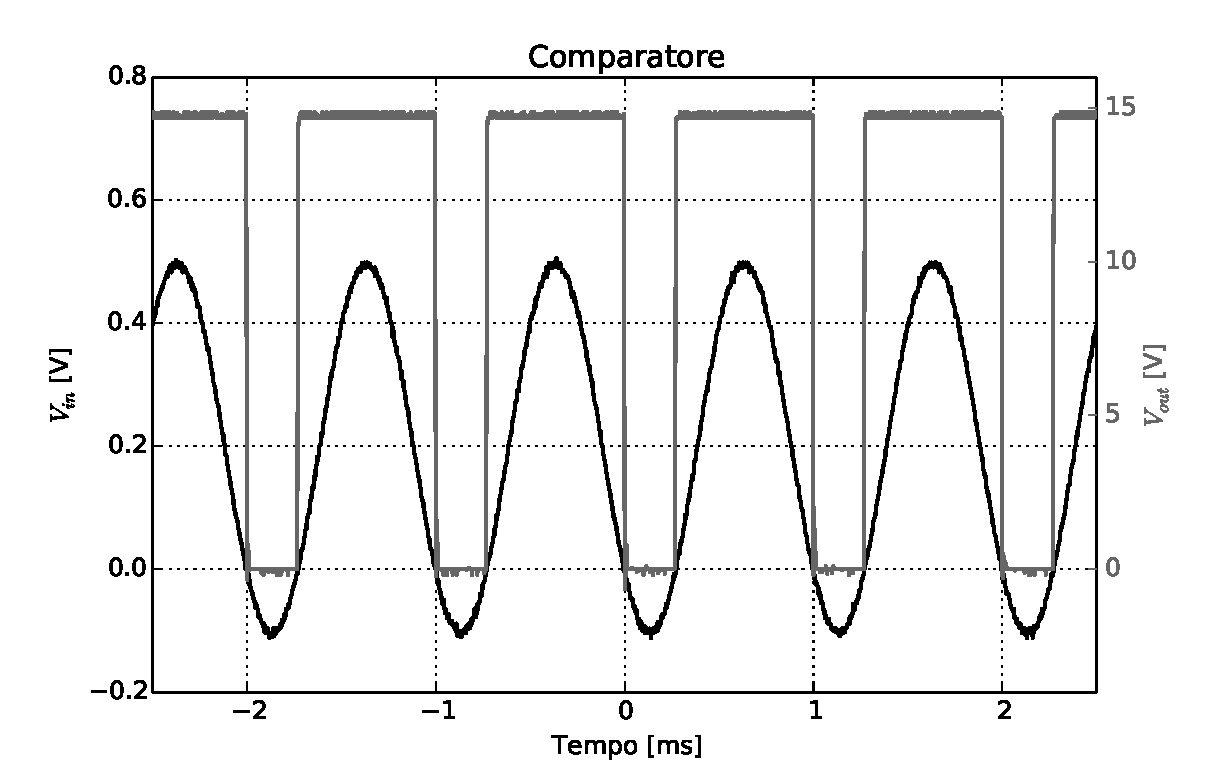
\includegraphics[width=0.75\textwidth]{figure/comp_graph.pdf}
    \caption{Il grafico mostra l'andamento del segnale in ustita ($V\ped{out}$), onda quadra, dal nostro comparatore LM311 fornito un segnale in ingresso sinusoidale. Come è possibile notare il segnale in uscita $V\ped{out}$ assume il valore di saturazione positiva $V\ped{sat}^+\,=\,\SI{}{\volt}$ ogni volta che $V\ped{in}\,\geq\,\SI{0}{\volt}$, mentre $V\ped{out}\,=\,\SI{0}{\volt}$ quando $V\ped{in}\,\leq\,\SI{0}{\volt}$. Inoltre è possibile osservare che il segnale in ingresso ha un offset di $\SI{0.2}{\volt}$.}
    \label{fig:comparatore_plot}
\end{SCfigure}
% Infine possimo notare la notevole amplificazione del comparatore. Infatti per tensioni in ingresso molto piccole, anche dell'ordine di millesimi di volt, si ha un amplificazione che permette di portare direttamente in saturazione positiva il comparatore. 

\subsection*{Trigger di Schmitt non inverente}

\begin{wrapfloat}{figure}{I}{0pt}
        \def\svgwidth{0.45\textwidth}
        \subimport{figure/}{trigger_schmitt.pdf_tex}
        \caption{Trigger di Schmitt. Il comparatore è usato in configurazione non invertente, inoltre è presente un ramo di retroazione positiva e non negativa.}
        \label{fig:trigger_schmitt}
\end{wrapfloat}

In questo paragrafo vogliamo realizzare un trigger di Schmitt non invertente, studiarne i valori di soglia, quindi ottenere $V\ped{sat}^+$ e $V\ped{sat}^-$ ed infine calcolarne l'isteresi.

Come prima cosa cerciamo di capire cosa sia un trigger di Schmitt. Il trigger di Schmitt è un particolare tipo di comparatore, è un circuito che consente di trasformare un segnale analogico ($V\ped{in}$) in un'uscita ($V\ped{out}$) che varia soltanto tra due valori di tensione, a seconda che l'ingresso superi una certa soglia ($V\ped{OH}$) o sia inferiore ad una seconda soglia ($V\ped{OL}$, più bassa di $V\ped{OH}$). Una delle sue applicazioni è la produzione di onde quadre a partire da un segnale sinusoidale, per questo è molto utilizzato nei circuiti logici per creare il segnale di sincronismo (clock).

Quindi il circuito che abbiamo realizzato è riportato in Figura \ref{fig:trigger_schmitt}. Le specifiche di questo circuito sono: la tensione di alimentazione positiva $V\ped{cc}^+$ ha un valore di $\SI{+15}{\volt}$, la tensione di alimentazione negativa $V\ped{cc}^-$ ha un valore di $\SI{-15}{\volt}$. La tensione $V_A\,\equiv\,V\ped{cc}^+$, e la resistenza $R_3\,=\,\SI{10}{\kilo\ohm}$ per lo stesso motivo illustrato nel paragrafo precedente.

Ora cerchiamo di capire come funziona tale circuito. Il trigger (grilletto) di Schmitt ha una tensione d'ingresso ($V\ped{in}$) ed una d'uscita ($V\ped{out}$). L'uscita può avere un valore o basso ($V\ped{sat}^-$) o alto ($V\ped{sat}^+$). Questo è dovuto al fatto che stiamo lavorando con un comparatore e non con un semplice amplificatore operazionale.
Nella configurazione non invertente quando l'entrata è al di sotto della tensione di soglia bassa ($V\ped{OL}$), l'uscita assume il valore ($V\ped{sat}^-$); quando l'entrata si trova al di sopra della tensione di riferimento ($V\ped{OH}$), l'uscita assume il valore alto ($V\ped{sat}^+$). Quando il valore in ingresso si trova compreso tra le due soglie ($V\ped{OH}$ e $V\ped{OL}$), l'uscita conserva il valore precedente finché l'entrata non sia variata sufficientemente da farne scattare il cambio (azione di trigger). Tutto questo processo va sotto il nome di isteresi del trigger di Schmitt e ha come scopo fondamentale quello di eliminare in modo consistente gli effetti dovuti al rumore elettrico o meno sul segnale in ingresso che deve essere analizzato dal comparatore.

Consideriamo un sistema simile, ma con soltanto una sola soglia d'ingresso. Un segnale in entrata rumoroso, di ampiezza prossima al valore di soglia, può oscillare rapidamente attorno a tale valore, facendo pertanto oscillare l'uscita tra il suo valore basso ed alto. Con il trigger di Schmitt, un segnale rumoroso vicino ad una soglia può causare una sola commutazione del valore d'uscita, dopo di che deve crescere verso l'altra soglia al fine di causare una ulteriore commutazione. Quindi grazie a questa configurazione si possono attenuare notevolmente le sbavature dovute al rumore del segnale in ingresso.

Quindi, fatte queste considerazioni, abbiamo deciso di adottare i seguenti valori per le resistenze $R_1$ e $R_2$:
\begin{equation}
        R_1\,=\,\SI{100}{\ohm} \qquad \text{e} \qquad R_2\,=\,\SI{100}{\kilo\ohm}
\end{equation}

Il risultato ottenuto è illustrato nel grafico riportato in Figura \ref{fig:schimtt_plot}.

\begin{figure}[H]
    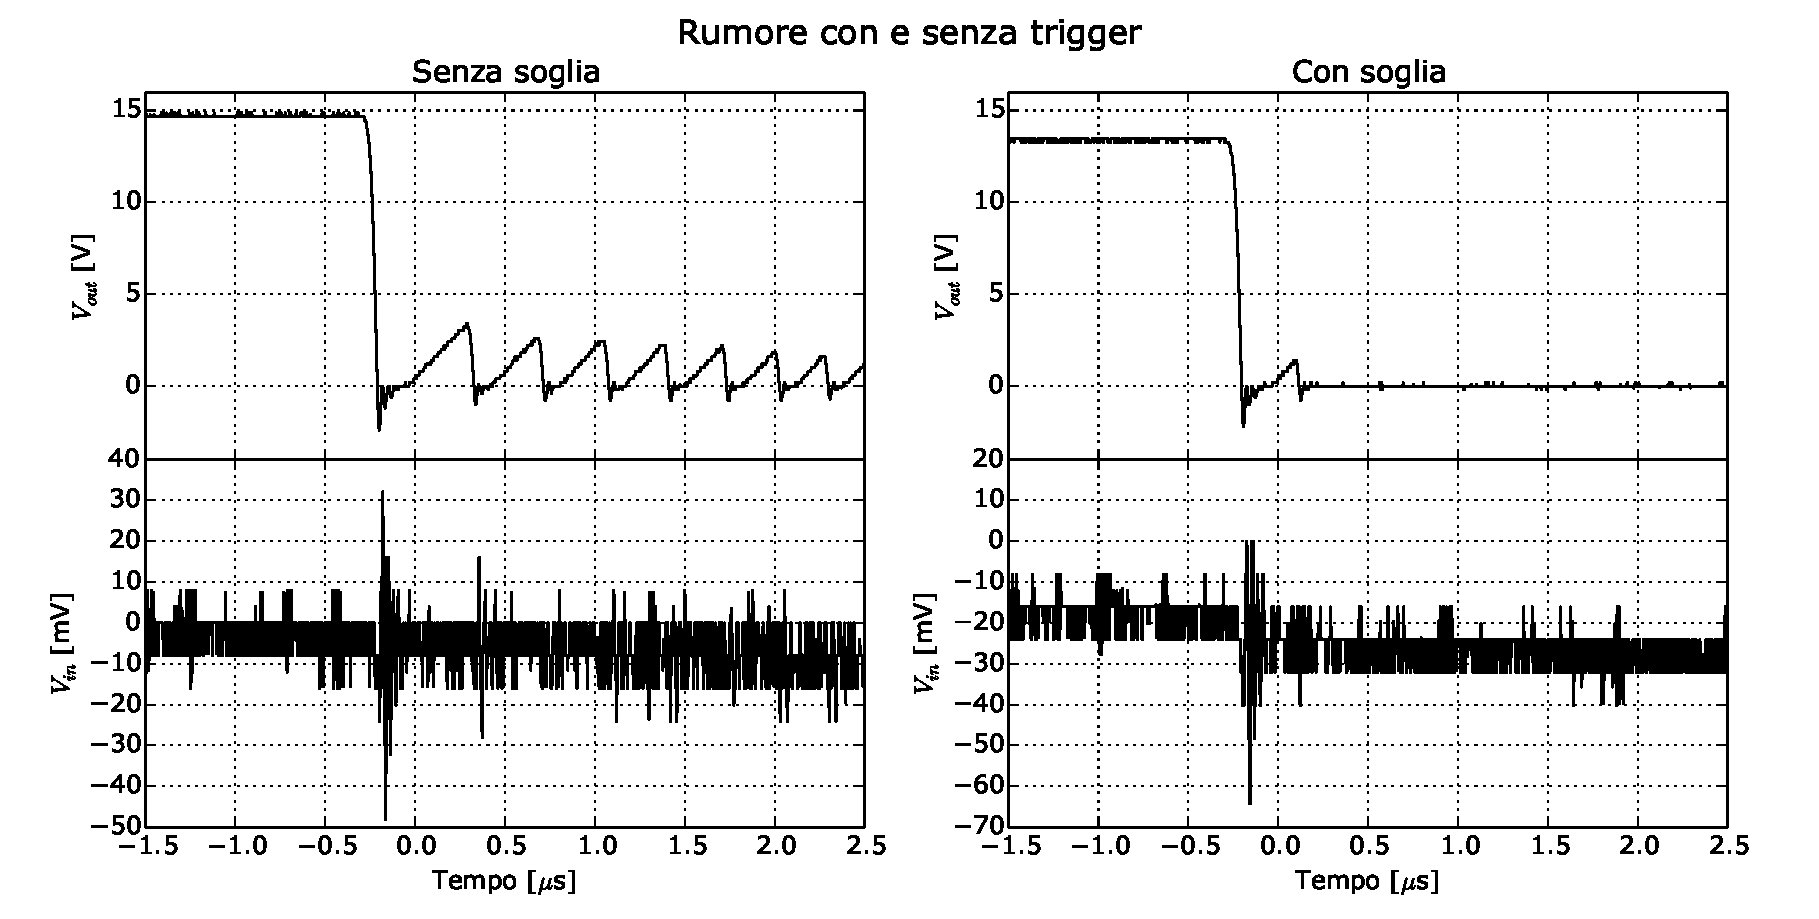
\includegraphics[width=\textwidth]{figure/trigger_graph.pdf}
    \caption{Questa immagine mostra un paragone tra il risultato che si otterrebbe con un comparatore senza trigger di Schmitt, nella figura a sinistra, e un comparatore dotato di questo trigger, figura a destra. Come si può chiaramente osservare nel caso in cui il comparatore sia dotato di trigger gli effetti del rumore sul segnale in uscita sono molto meno visibili. Questo è merito della doppia soglia che permette di non far scattare il comparatore appena il segnale in ingresso assume valore positivo o negativo, ma come già spiegato, ammette un range di tensioni, che sono un intorno dello zero, per le quali il segnale in output mantiene il suo valore, positivo o negativo che fosse. Il nostro intervallo di accettazione è:$V\ped{OL}\,=\,(-12.9\pm0.1)\SI{}{\milli\volt}$, soglia bassa e $V\ped{OH}\,=\,\SI{0}{\milli\volt}$, soglia alta.}
    \label{fig:schmitt_plot}
\end{figure}

Dai grafici riportati in Figura \ref{fig:schmitt_plot} possiamo visualizzare quanto spiegato in precedenza. Ovvero nella prima immagine si può chiaramente osservere come il comparatore scatta, quindi varia il valore della tensione di offset ($V\ped{out}$) tra i due valori di saturazione permessi ($V\ped{sat}^+$ e $V\ped{sat}^-$), ogniqualvota il senale in ingresso ($V\ped{in}$) passa da valori positivi a negativi. Queste variazioni sono dovute principalmente alrumore di fondo che perturba il segnale in ingresso. Al contraio se dotiamo il comparatore del trigger di Schmitt possiamo attenuare enormemente gli effetti del rumore in input. Infatti impediamo che il comparatore vari la tensione di offset ogni volta che $V\ped{in}$ interseca l'asse delle ascisse.
Infatti, come spiegato in precedenza, abbiamo due valori di soglia $V\ped{OL}\,=\,(-12.9\pm0.1)\SI{}{\milli\volt}$, soglia inferiore, $V\ped{OH}\,=\,\SI{0}{\milli\volt}$, soglia maggiore, e fintanto che $V\ped{in}$ appartiene a questo intervallo la tensione di output mantiene il valore di saturazione positiva se $V\ped{in}\,\geq\,V\ped{OH}$, di saturazione negativa se $V\ped{in}\,\leq\,V\ped{OL}$.

Tutto quello detto fino a questo punto può essere riassunto nel grafico riportato in Figura \ref{fig:isteresi_plot}, che riassume il comportamento del comparatore quindi di $V\ped{out}$ a seconda dei valori di tensione assunti dall'input ($V\ped{in}$).

\begin{SCfigure}[0.8][h]
    \centering
    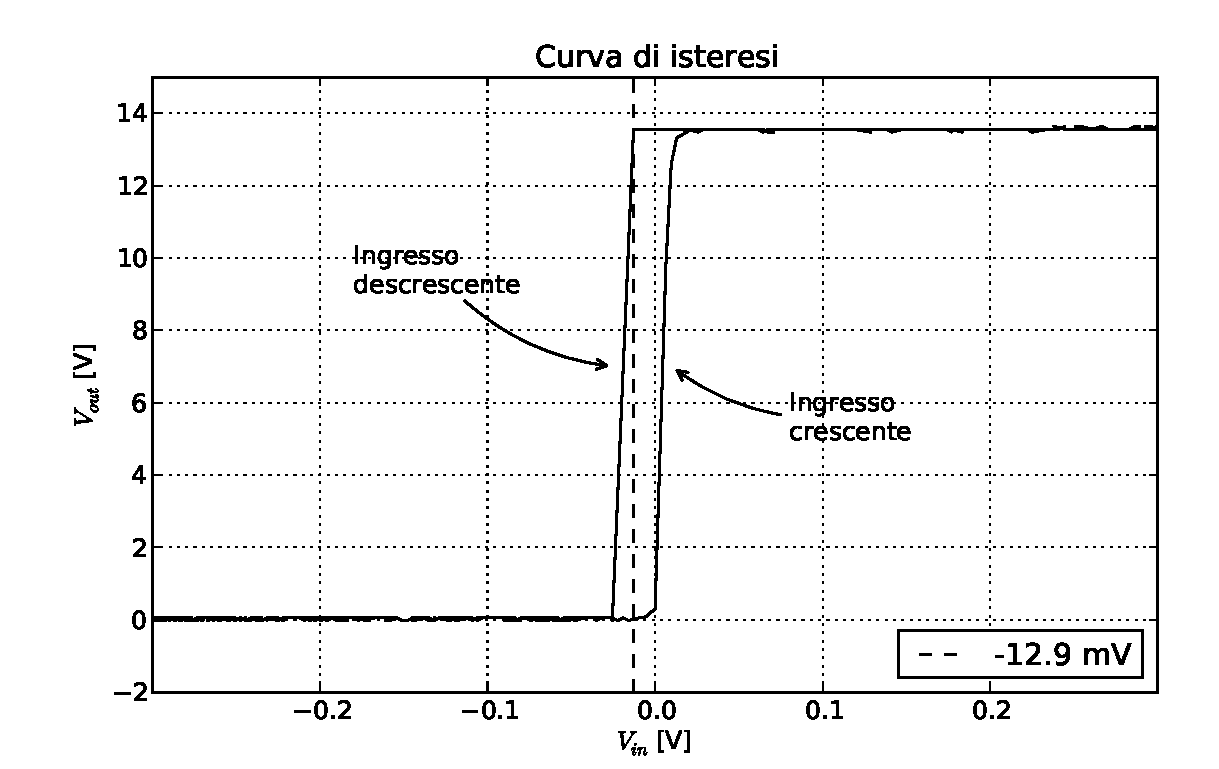
\includegraphics[width=0.8\textwidth]{figure/isteresi.pdf}
    \caption{Questo grafico mostra come varia la differenza di potenziale in output ($V\ped{out}$) al ariare della differenza di potenziale in ingresso ($V\ped{in}$). In particolare la larghezza del ciclo, detto appunto ciclo di isteresi, è la larghezza del nostromintervallo di accettazione, ovvero la differenza di potenziale tra $V\ped{OH}$, ingresso crescente e $V\ped{OL}$, ingresso decrescente.}
    \label{fig:isteresi_plot}
\end{SCfigure}

\subsection*{Oscillatore a rilassamento}

\begin{wrapfloat}{figure}{I}{0pt}
        \def\svgwidth{0.45\textwidth}
        \subimport{figure/}{oscillatore.pdf_tex}
        \caption{Oscillatore a rilassamento. Prestare attenzione che l'ampificatore operazionale utilizzato è il comparatore LM311.}
        \label{fig:oscillatore}
\end{wrapfloat}

In questo paragrafo vogliamo studiare un oscillatore a rilassamento, ovvero, sfruttando il circuito riportato in Figura \ref{fig:oscillatore}, andremo a studiare il segnale in uscita dall'amplificatore operazionale ($V\ped{out}$) e ai capi del condensatore ($V_c$) ne trarremo le dovute conclusioni. Faccimo presente che per questo circuito è stato utilizzato l'amplificatore operazionale UA741 e non il comparatore LM311.

Come primo passo cerchiamo di capire cosa sia un oscillatore a rilassamento. Gli oscillatori a rilassamento sono dispositivi eletronici in grado di emettere seganli elettrici di varie forme non sinusoidali. Possono emettere, per esempio, onde quadre o onde a dente di sega.
La caratteristica fondamentale del circuito è che idealmente entrambi gli ingressi sono collegati al conume, tuttavia nel nostro caso per l'ingresso non invertente ($V^+$) il collegamento avviene grazie ad una resistenza, che è un componente lineare. Alcontrario per l'ingresso invertente ($V^-$) il collegamento avviene tramite un condensatore, che è un componente non lineare. Ed è proprio il componente non lineare che periodicamente, scaricando l'energia accumulata, crea una diffrenza di potenziale notevole in uscita, tale da portare in saturazione negativa o positiva l'amplificatore operazionale.
Sostenzialmente possimo immaginare il circuito in Figura \ref{fig:oscillatore} come un trigger di Schmitt. All'inizio l'OPAMP amplifica la tensione di offset (V\ped{os}). Quindi in un primo momento la tensione di output (V\ped{out}) assume valore positivo o per essere precisi si porta in saturazione positiva ($V\ped{sat}^+$) e grazie al ramo di retroazione negativo permette la carica del condensatore. Ad un certo punto l'OPAMP si porta in saturazione negativa overo l'output assume un valore corrispondente a ($V\ped{sat}^-$) e il condensatore, sempre per effetto della retroazione negativa comincia a scaricarsi. Questo ciclo che prevede il passaggio dell'output da valori di tensioni positivi a negativi, che portano quindi il condensatore a cicli di carica e scarica, si ripete all'infinito.

Le specifiche del circuito realizzato sono: la tensione di alimentazione positiva $V\ped{cc}^+$ ha un valore di $\SI{+15}{\volt}$, la tensione di alimentazione negativa $V\ped{cc}^-$ ha un valore di $\SI{-15}{\volt}$. I valori di resistenza usati sono i seguenti: $R_1\,e\,R_2\,=\,\SI{10}{\kilo\ohm}$ mentre per $R$ abbiamo usato un trimer in modo da poter variare la frequanza delle oscillazioni a nostro piacimento. La capcità del condensatore vale $C\,=\,\SI{100}{\nano\farad}$

Possimo variare la frequenza delle oscillazioni a nostro piacimento in quanto abbiamo studiato che:
\begin{equation}
        \tau\ped{teo}\,=\,2RC\,\ln \left(1+\frac{2R_1}{R_2}\right)\,=\,(\pm)\SI{}{\second}  
\end{equation}
dove con $\tau\ped{teo}$ indichiamo il tempo caratteristico di carica del condensatore, teorico. Con $R$ indichiamo la resistenza variabile, con $C$ facciamo riferimento alla capacità del condensatore e $R_1$ e $R_2$ sono le resistenze di cui sopra.

\subsection*{Interruttore crepuscolare}

\begin{wrapfloat}{figure}{O}{0pt}
        \def\svgwidth{0.45\textwidth}
        \subimport{figure/}{crepuscolare.pdf_tex}
        \caption{circuito rappresentante l'interruttore crepuscolare, che come possiamo notare è composto da tre blocchi. Il fototransistor, la sorgente di corente costante ed il comparatore.}
        \label{fig:interruttore}
\end{wrapfloat}

In questo ultimo paragrao ci occupiamo della progettazione e della realizzazione di un interruttore crepuscolare. Prima di tutto aniamo a spiegare che cosa sia un interruttore crepuscolare: è un componente elettronico che permette l'attivazione automatica di un circuito di illuminazione una volta raggiunta una soglia minima di illuminazione dell'ambiente. Tale soglia può essere impostata a piacere dall'operatore.

Detto questo sfruttiamo il circuito riportato in Figura \ref{fig:interruttore} per spiegare i passaggi che ci hanno portato alla realizzazione dell'interruttore repuscolare. Come si può notare lo stadio di ingresso del nostro circuito è costituito da un fototransistor, che è un dispositivo elettronico che permette di trasformare la radiazione elettromagnetica, in questo caso la radiazione luminosa, in un segnale elettrico di corrente con la presenza di un opportuno potenziale ai suoi estremi.
Il secondo stadio del nosro circito è costituito da un amplificatore operazionale UA741. Con questo amplificatore vogliamo appunto amplificare il segnale in ingresso. Inoltre possiamo osservare che la sua configurazione è quella di una sorgente di corente costante infatti. Per questo motivo in uscita da questo stadio avremo un intensità di corrente molto maggiore a quella in ingresso. Tutto questo ci è permesso se imponiamo un valore della resistenza $R_3$ molto elevato, come ad esempio $\SI{1}{\mega\ohm}$, in modo che grazie ad una semplice analisi circuitale si possa ottenere che il segale in uscita vale:
\begin{equation}
        V\ped{out}\,=\,-I\,R_3 \qquad \text{dove con $I$ indichiamo la corrente entrante nell'amplificatore operazionale.}
\end{equation}
e pertanto anche la corrente in uscita risulta amplificata, naturalmente se $R_1\,\leq\,R_3$.
Per questo motivo le specifiche del secondo stadio del nostro circuito sono le seguenti: la tensione di alimentazione positiva $V\ped{cc}^+$ ha un valore di $\SI{+15}{\volt}$, la tensione di alimentazione negativa $V\ped{cc}^-$ ha un valore di $\SI{-15}{\volt}$. L'ingresso non invertente è collegato al comune e $R_3\,=\,\SI{1}{\mega\ohm}$.
Per concludere andiamo ad analizzare il terzo ed ultimo stadio del nostro circuito. Questa parte è costituita principalmente da un comparatore LM311. Come prima oservazione possiamo dire che l'ingresso invertente è collegato ad un trimer, ai cui capi è applicata una differenza di potenziale di $\SI{+15}{\volt}$, in modo che l'operatore possa scegiere la soglia a cui far scattare il comparatore. Quindi è un controllo manuale per il settaggio del circuito. Proseguendo possiamo notare che come comparatore svolge la semplice funzione descritta anche nel primo paragrafo di questo elaborato. Ovvero quando $V^+$ (ingreso non invertente) è maggiore di $V^-$ (ingresso invertente) il comparatore si comporta come un interruttore aperto. Pertanto l'output del comparatore ($V\ped{out}$) assumerà un valore di tensione $V\ped{sat}^+$ e quindi il led nel ramo di pull-up non si accenderà in quanto in quel ramo non scorre corrente. Nel momento in cui $V^+\,\leq\,V^-$ allora ilcomparatore si comporta come un interruttore chiuso e porta loutput a una tesione nulla. Quindi nel ramo di pull-up scorre corrente e il led si illumina.
Infine per completezza riportiamo le specifiche di questo ultimo stadio del nostro circuito. La tensione di alimentazione positiva $V\ped{cc}^+$ ha un valore di $\SI{+15}{\volt}$, la tensione di alimentazione negativa $V\ped{cc}^-$ ha un valore di $\SI{-15}{\volt}$. I valori di resistenza sono i seguenti: $R_1\,=\,\SI{10}{\kilo\ohm}$, $R_2\,=\,\SI{100}{\kilo\ohm}$ ed infine $R_4\,=\,\SI{1}{\kilo\ohm}$. 

Questo quindi è, a grandi linee, il ragionamento che ci ha portato alla realizzazione di questo interruttore crepuscolare, del quale, tra l'altro, abbiamo testato il corretto funzionmento verificando che il led si accendesse quando l'intesità luminosa dell'ambiente non era sufficientemente elevata. Tutto ha funzionato corretttamente.
